%! Author = Leonhard Gahr <leonhard.gahr@gmail.com>
%! Date = 22/01/20
%! Info = Tx000_template

\documentclass[
ngerman, % new German spelling
a4paper, % paper size
%twoside, % Zweiseitiger Druck (rechts/links)
12pt,
pdftex,
disable % disable Todos
]{report}

\usepackage[utf8]{inputenc} % UTF-8 coding
\usepackage[english,german]{babel}

\usepackage{bericht}
\usepackage{lipsum}

\makenoidxglossaries
\glstocfalse
\setabbreviationstyle{long-short}

%! Author = Leonhard Gahr <leonhard.gahr@gmail.com>
%! Date = 22/01/20
%! Info = Tx000_template

\newglossaryentry{visual-studio}
{
  name=Visual Studio,
  description={Programmierumgebung zum Entwickeln von Software}
}
\newglossaryentry{frontend}
{
  name=Frontend,
  plural=Frondends,
  description={Darstellungsebene einer Anwendung}
}
\newglossaryentry{backend}
{
  name=Backend,
  description={Ausführende Logik einer Anwendung, die im Hintergrund agiert}
}

\newglossaryentry{full-stack}
{
  name=Full-Stack,
  description={Entwicklung von Anwendung im \gls{frontend} sowie \gls{backend}}
}

% \newabbreviation[\glslongpluralkey=long_pl, \glsshortpluralkey=short_pl]{name}{presentation}{long-presentation}
\newabbreviation[\glslongpluralkey=Virtuellen Maschinen, \glsshortpluralkey=VMs]{vm}{VM}{Virutelle Maschine}
\newabbreviation[\glslongpluralkey=Abkürzungen, \glsshortpluralkey=Abk-en]{Abk}{Abk.}{Abkürzung}
\newabbreviation{OP EX PH}{Opcenter EXPH}{Opcenter Execution Pharma}
\newabbreviation{MES}{MES}{Manufacturing Execution System}
\newabbreviation{UI}{UI}{Benutzeroberfläche}
\newabbreviation{VB}{VB}{Visual Basic}
\newabbreviation{ESXi}{ESXi}{Elastic Sky X Integrated}
\newabbreviation[\glslongpluralkey=Process Instructions, \glsshortpluralkey=PIs]{PI}{PI}{Process Instruction}
\newabbreviation[\glslongpluralkey=Dynamic Link Libraries, \glsshortpluralkey=DLLs]{dll}{DLL}{Dynamik Link Library}
\newabbreviation{SQL}{SQL}{Structured Query Language}



% Information of the paper

\newcommand{\Autor}{Leonhard Gahr}
\newcommand{\MatrikelNummer}{8858650}
\newcommand{\Kursbezeichnung}{TINF18B4}

\newcommand{\FirmenName}{Siemens AG}
\newcommand{\FirmenStadt}{Karlsruhe}
\newcommand{\FirmenLogoDeckblatt}{
\includegraphics[width=5cm]{img/sie-logo.png}}

\newcommand{\BetreuerFirma}{Prof. Kai Becher}
\newcommand{\BetreuerDHBW}{Prof. Dr. Jörn Eisenbiegler}


\newcommand{\Was}{Studienarbeit}

\newcommand{\Titel}{MES Portal}
\newcommand{\AbgabeDatum}{14. September 2020}

\newcommand{\Abschluss}{Bachelor of Science}

\newcommand{\Studiengang}{Angewandte Informatik}

\hypersetup{
pdfauthor={\Autor},
pdftitle={\Titel},
pdfsubject={\Was}
}

\newenvironment{abstractpage}
{\cleardoublepage\vspace*{\fill}\thispagestyle{empty}}
{\vfill\cleardoublepage}
\newenvironment{myabstract}[1]
{\bigskip\selectlanguage{#1}
\begin{center}
    \bfseries\abstractname
\end{center}}
{\par\bigskip}

\bibliography{bericht}

% REMOVE ON RELEASE
\usepackage[12hr]{datetime}

\setstretch{1.25}
\begin{document}
\begin{titlepage}
  \begin{center}
    \vspace*{-2cm}
    \FirmenLogoDeckblatt\hfill
\includegraphics[width=4cm]{img/dhbw-logo}\\[2cm]
    {\Huge \Titel}\\[1cm]
    {\Huge\scshape \Was}\\[1cm]
    {\large für die Prüfung zum}\\[0.5cm]
    {\Large \Abschluss}\\[0.5cm]
    {\large des Studiengangs \Studiengang}\\[0.5cm]
    {\large an der}\\[0.5cm]
    {\large Dualen Hochschule Baden-Württemberg Karlsruhe}\\[0.5cm]
    {\large von}\\[0.5cm]
    {\large\bfseries \Autor}\\[1cm]
    {\large Abgabedatum \AbgabeDatum}
    \vfill
  \end{center}
  \begin{tabular}{l@{\hspace{2cm}}l}
    Matrikelnummer                & \MatrikelNummer  \\
    Kurs                          & \Kursbezeichnung \\
    Ausbildungsfirma              & \FirmenName      \\
                                  & \FirmenStadt     \\
    Betreuer der Ausbildungsfirma & \BetreuerFirma   \\
    Gutachter der Studienakademie & \BetreuerDHBW    \\
  \end{tabular}
\end{titlepage}

%! Author = Leonhard Gahr <leonhard.gahr@gmail.com>
%! Date = 22/01/20
%! Info = Tx000_template

% In Bachelorarbeiten muss eine schriftliche Erklärung abgegeben werden.
% Hierin bestätigen die Studierenden, dass die Bachelorarbeit, etc.
% selbständig verfasst und sämtliche Quellen und Hilfsmittel angegeben sind. Diese Erklärung
% bildet das zweite Blatt der Arbeit. Der Text dieser Erklärung muss auf einer separaten Seite
% wie unten angegeben lauten.

\newpage
\thispagestyle{empty}
\begin{framed}
    \begin{center}
        \Large\bfseries Erklärung
    \end{center}
    \medskip
    \noindent
    % siehe §5(3) der \enquote{Studien- und Prüfungsordnung DHBW Technik} vom 29.9.2017
    Ich versichere hiermit, dass ich meine \Was\ mit dem Thema:
    \enquote{\Titel}
    selbstständig verfasst und keine anderen als die angegebenen Quellen und Hilfsmittel benutzt habe. Ich versichere zudem, dass die eingereichte elektronische Fassung mit der gedruckten Fassung übereinstimmt.\\[3cm]
    \underline{\hspace{4cm}}\hfill\underline{\hspace{6cm}}\\
    Ort~~~~~Datum\hfill Unterschrift\hspace{4cm}
\end{framed}

\endinput


% abstracts
\begin{abstractpage}
  \begin{myabstract}{german}
    Für das Siemens Produkt \gls{OP EX PH} existiert die Anwendung MES Portal, welche auf der Programmiersprache \gls{VB} 6 basiert. Zwei Module des Portals sind der Test Manager und der Workorder Planner. Diese werden aufgrund der veralteten Technologie in eine moderne, webbasierte Technologie portiert. Als neue Technologie soll das Framework Radzen verwendet werden. Bei der Entwicklung ergeben sich Schwierigkeiten, durch welche die Entwicklung nur verzögert fortgesetzt und nicht abgeschlossen werden kann.
  \end{myabstract}

  \begin{myabstract}{english}
    The MES Portal is an application for the Siemens product \gls{OP EX PH}, which is written in the programming language \gls{VB}6. Two modules of that portal are the Test Manager and the Workorder Planner. As \gls{VB}6 is an outdated technology, these modules will be rewritten in a new, web based technology. The Radzen framework suits this use case. Technical problems delayed the development and the development could not be completed. A follow up project will be planned to complete the implementation
  \end{myabstract}
\end{abstractpage}

\tableofcontents
\listoftables
\listoffigures
\lstlistoflistings

\printnoidxglossary[type=main, title={Glossar}]
\printnoidxglossary[type=\acronymtype, title={Abkürzungsverzeichnis}]



% begin of chapters
%! Author = Leonhard Gahr <leonhard.gahr@gmail.com>
%! Date = 22/01/20
%! Info = Tx000_template

\chapter{Einleitung}
\section{Projektbeschreibung}

%! Author = Leonhard Gahr <leonhard.gahr@gmail.com>
%! Date = 22/01/20
%! Info = Tx000_template

\chapter{Grundlagen - das MES Portal}
Um \gls{OP EX PH} zu steuern, werden viele Tools mitgeliefert, die unterschiedliche Funktionen erfüllen, z. B. das Anlegen neuer \glspl{PI} oder Starten von Arbeitsaufträgen. Manche Abläufe sind dabei so komplex, dass sie das Verwenden von mehreren Tools voraussetzen, die jeweils eine Authentifizierung erfordern und es müssen immer dieselben Abläufe ausgeführt werden. Für diese Aktivitäten wurde das MES Portal eingeführt, um solch grundlegende Arbeitsabläufe zu vereinfachen und teilweise zu automatisieren.\\
\Cref{fig-mes_portal_overview} zeigt eine reduzierte Version des Hauptmenüs des MES Portals. Hier ist u. a. das Modul Test Manager zu erkennen (\Cref{sec-test_manager}).

\begin{figure}[htbp]
  \centering
  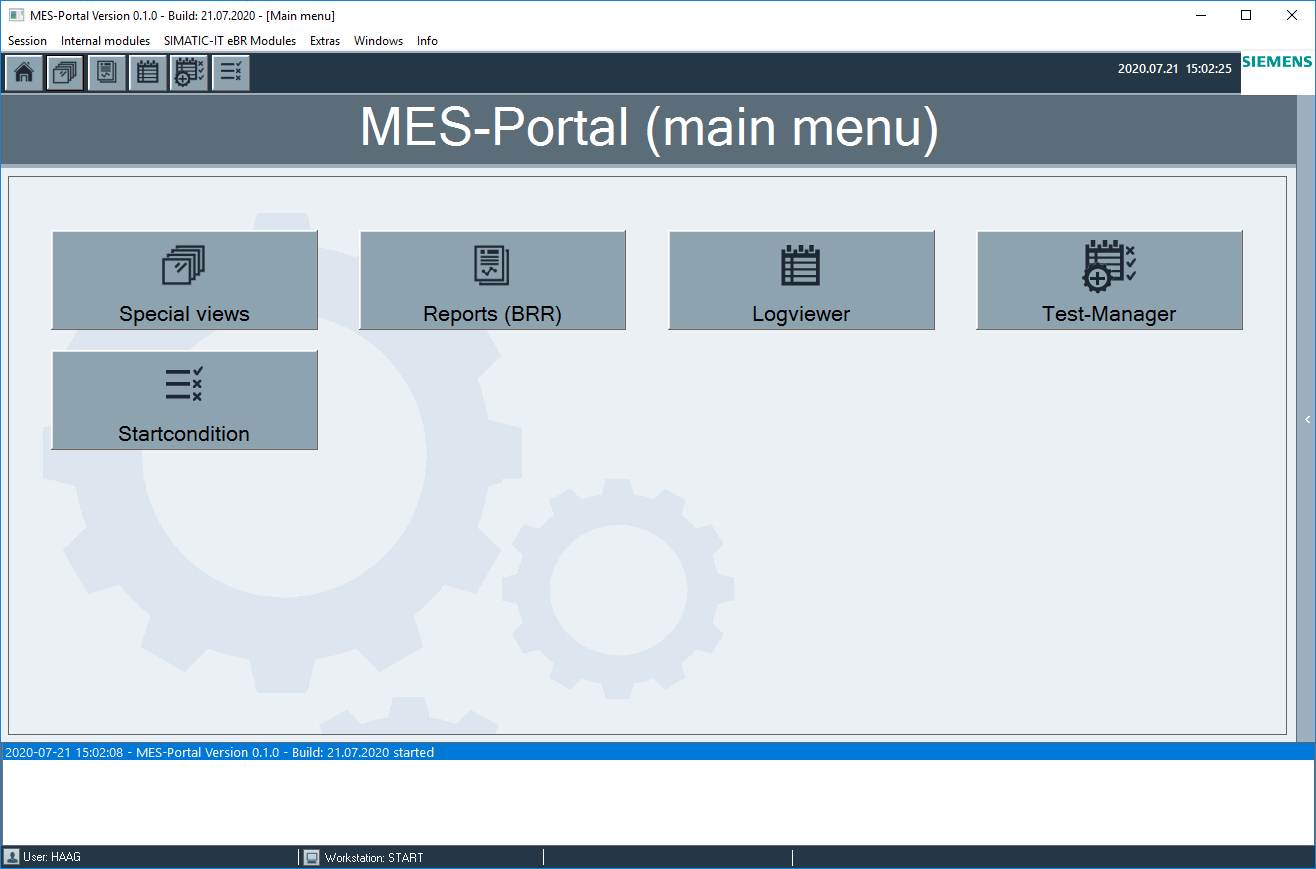
\includegraphics[width=.7\textwidth]{img/mes-portal_overview}
  \caption{\label{fig-mes_portal_overview}MES Portal - Hauptmenü}
\end{figure}

\section{Test Manager}\label{sec-test_manager}
Der Test Manager (\Cref{fig-mes_portal_test-manager}) bietet Funktionen zum automatisierten Testen von \glspl{PI}. Dabei werden die Funktionen unterteilt in \textbf{\nameref{sub_sec-test_manager-basics}}, die dem eigentlichen Ziel, dem Testen von Arbeitsaufträgen, dienen und \textbf{\nameref{sub_sec-test_manager-advanced}}, die der Benutzerfreundlichkeit dienen und das Verwenden des Test Managers erleichtern.

\begin{figure}[htbp]
  \centering
  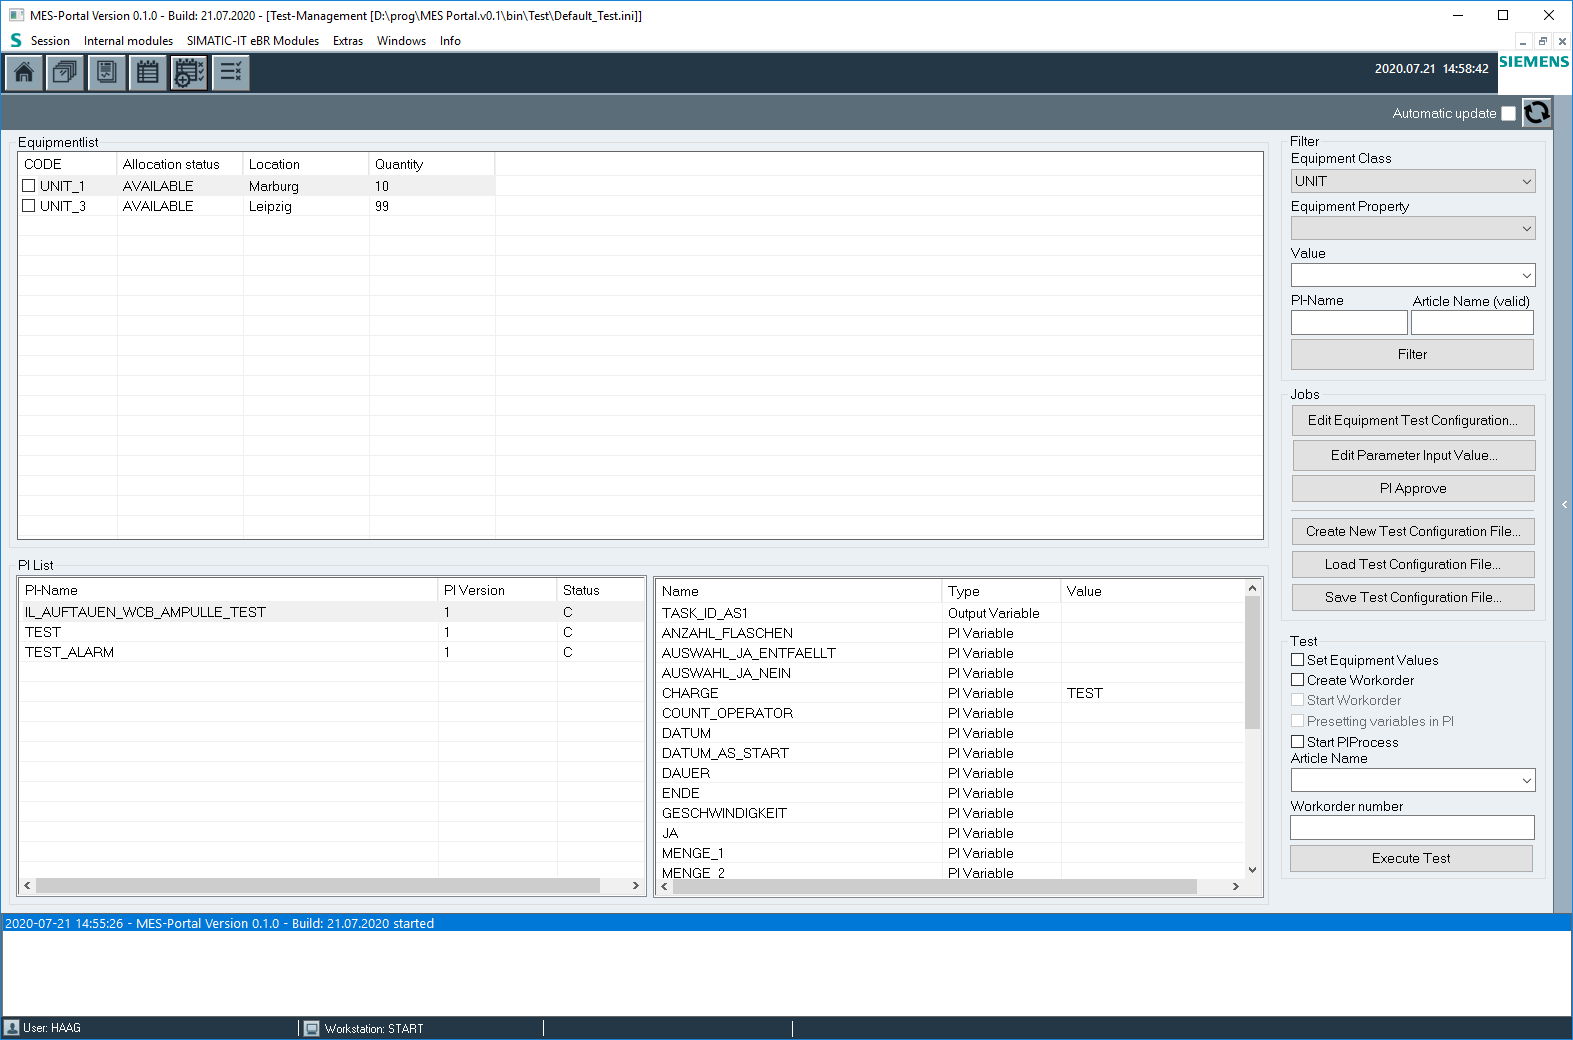
\includegraphics[width=\textwidth]{img/mes-portal_test-manage}
  \caption{\label{fig-mes_portal_test-manager}MES Portal - Test Manager (alt)}
\end{figure}

\newpage\subsection{Unterschied PI und Arbeitsauftrag}
Im Zusammenhang mit dem Test Manager kommen die Begriffe \gls{PI} und Arbeitsauftrag oft eng zusammen vor. Der Unterschied liegt in der Herkunft. Eine \gls{PI} wird von einem Nutzer definiert und beschreibt bestimmte Arbeitsschritte (\glsentrylong{PI}) auf einer konstanten Basis. Eine \gls{PI} wird im Allgemeinen nicht verändert.\\
Ein Arbeitsauftrag hingegen ist die ausführende Instanz einer \gls{PI}. Dieses Verhältnis ist äquivalent mit einem Objekt in der Objektorientierten Programmierung zu seiner Instanz. Eine \gls{PI} ist die Definition des Objekts und ein Arbeitsauftrag ist eine von womöglich vielen Instanzen dieses Objekts.\\
Wie ein Objekt auch kann eine \gls{PI} Variablen besitzen, die bei der Ausführung des Arbeitsauftrages gesetzt werden.

\subsection{Grundfunktionen}\label{sub_sec-test_manager-basics}
Dabei besteht der Prozess aus fünf Schritten:
\begin{enumerate}
\item Equipment Variablen setzen
\item Arbeitsauftrag erstellen
\item Arbeitsauftrag starten
\item \gls{PI} Variablen setzen
\item PIProcess starten
\end{enumerate}

\subsubsection{Equipment Variablen setzen}
In diesem Schritt werden die konfigurierten Werte für die Equipments in die Datenbank geschrieben, auf die der Arbeitsauftrag später zugreifen wird.

\subsubsection{Arbeitsauftrag erstellen}
Hier wird über die Schnittstelle zu \gls{OP EX PH} ein Arbeitsauftrag mit einer gegebenen Arbeitsauftragsnummer im System angelegt.

\subsubsection{Arbeitsauftrag starten}
Der erstellte Arbeitsauftrag wird gestartet.

\subsubsection{PI Variablen setzen}
Die konfigurierten Variablen werden in der Datenbank zu dem Arbeitsauftrag hinzugefügt.

\subsubsection{PIProcess starten}
Startet das Programm PIProcess, mit dem der Arbeitsauftrag überwacht werden kann und ggf. manuelle Eingaben getätigt werden können.

\subsection{Zusatzfunktionen}\label{sub_sec-test_manager-advanced}
Die Zusatzfunktionen des Test Managers bestehen aus den Kategorien \textbf{Filter} und \textbf{Jobs}, die sich auf der rechten Seite der \Cref{fig-mes_portal_test-manager} befinden.

\subsubsection{Filter}
Die Filter beziehen sich teilweise auf die Equipments, aber auch auf die \glspl{PI}.\\
Equipments können nach der Klasse gefiltert werden. Die Klasse ist ein Bezeichner für die Art des Equipments (z. B. eine Maschine). Außerdem besitzen Equipments Eigenschaften in der Datenbank (z. B. \enquote{Allocation Status} oder Standort). Nach diesen Eigenschaften kann ebenfalls gefiltert werden.\\
\glspl{PI} können nach Namen oder nach dem Produkt gefiltert werden, das sie produzieren.

\subsubsection{Jobs}
Unter der Kategorie Jobs befinden sich einige Funktionen, die die Arbeit mit den einzelnen \glspl{PI} erleichtern. Die drei Knöpfe \enquote{Create New-}, \enquote{Load-} und \enquote{Save Test Configuration...} dienen dem Speichern der aktuellen Einstellungen, um die Arbeit an der jeweiligen \gls{PI} wieder aufnehmen zu können.\\
Die Funktionen \enquote{Edit Equipment Test Configuration...} und \enquote{Edit Parameter Input Value...} öffnen jeweils einen Dialog, in dem die Werte für alle aktuell sichtbaren Equipments bzw. \gls{PI}-Variablen auf einmal gesetzt werden können. Mit \enquote{PI Approve} wird der Status der ausgewählten \gls{PI} auf \enquote{Approved} gesetzt, damit sie ausgeführt werden kann.

\newpage\section{Workorder Planner}
Um eine bessere Übersicht über geplante oder bereits abgeschlossene Arbeitsaufträge zu erhalten, zeigt der Workorder Planner alle existierenden Arbeitsaufträge in chronologischer Reihenfolge in einem Kalender an (\Cref{fig-mes_portal_workorder-planner}). Da mehrere Arbeitsaufträge gleichzeitig in \gls{OP EX PH} erfasst und ausgeführt werden können, werden die Aufträge nach der Anlage gruppiert, in der sie ausgeführt werden. In \gls{OP EX PH} werden Arbeitsaufträge ohne Gruppierung in einer Tabelle angezeigt, die keine gute Übersicht über Start- und Endzeitpunkt aller Arbeitsaufträge gibt, um z. B. die Auslastung einer Produktionsanlage einsehen zu können.
\begin{figure}[htbp]
  \centering
  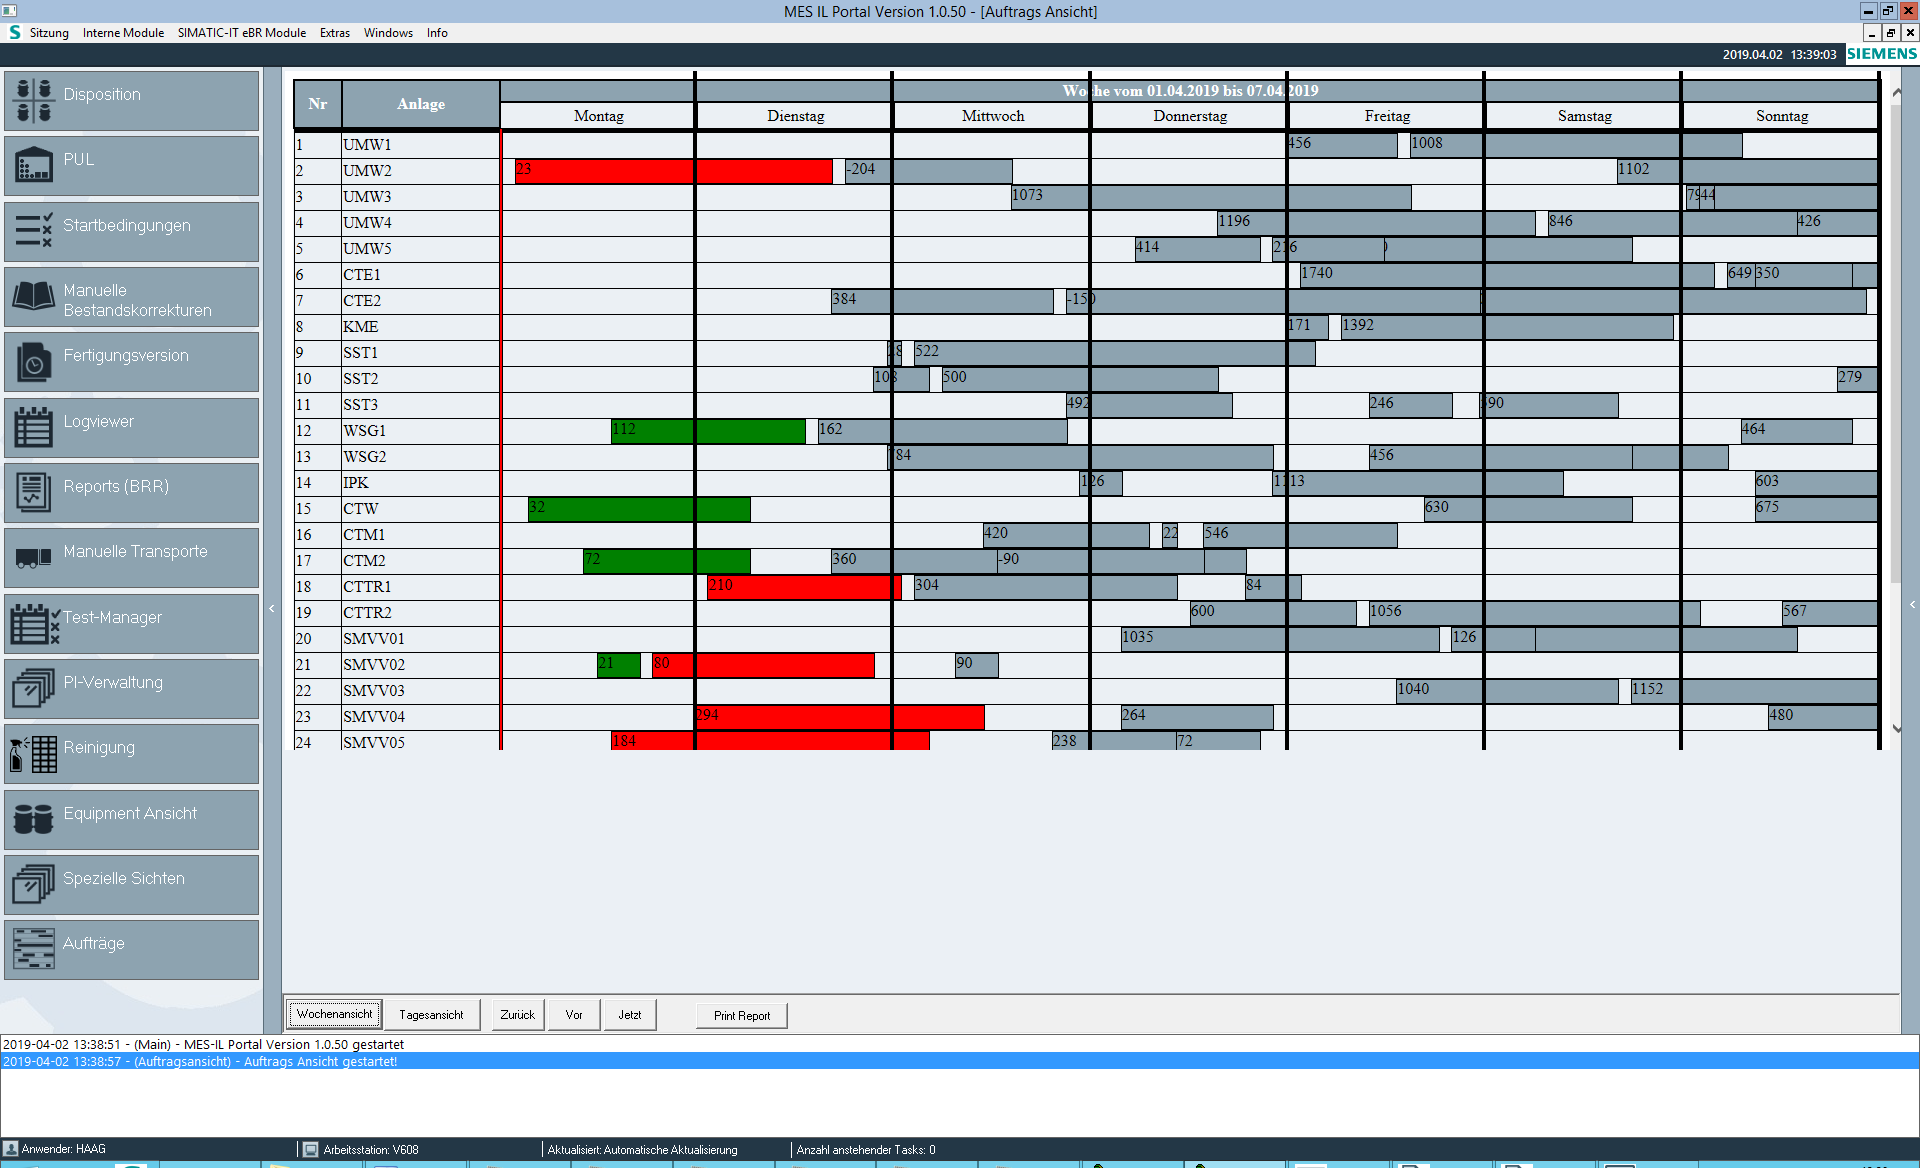
\includegraphics[width=\textwidth]{img/mes-portal_workorder-planner}
  \caption{\label{fig-mes_portal_workorder-planner}MES Portal - Workorder Planner (alt)}
\end{figure}

\noindent Die angezeigten Daten zu den Arbeitsaufträgen werden aus der \gls{OP EX PH} Datenbank bezogen. In dieser Datenbank werden jedoch keine Daten zum geschätzten Abschlusszeitpunkt eines Arbeitsauftrages abgelegt. Diese Daten kommen aus einem System von SAP, das diese Information in der Datenbank in einem benutzerdefinierten Feld \enquote{XFIELD09} einträgt. Die \enquote{XFields} sind zehn durchnummerierte, standardmäßig leere Spalten zu jedem Arbeitsauftrag in der Datenbank.
%! Author = Leonhard Gahr <leonhard.gahr@gmail.com>
%! Date = 22/01/20
%! Info = Tx000_template

\chapter{Umsetzung}
Zu Beginn des Projekts stellt sich heraus, dass es zeitliche Komplikationen bei der Umsetzung geben wird. Aufgrund einer verkürzten Praxisphase sowie zusätzlicher Abwesenheiten, beschränkt sich diese Praxisphase auf 30 Arbeitstage, von denen ca. 18 Tage für andere Arbeiten investiert werden müssen. Daher beschränkt sich die Umsetzung des Test Managers auf die Grundfunktionen, die in \Cref{sub_sec-test_manager-basics} beschrieben sind.\\
Die Umsetzung wird strukturiert in die Schritte \textbf{Einarbeitung} und \textbf{Entwicklung}, da mit neuen Technologien gearbeitet wird.
\section{Einarbeitung}
Die Einarbeitung besteht aus der Analyse des \gls{VB}6-Codes und des \glspl{frontend} (\Cref{fig-mes_portal_test-manager}), des bestehenden Test Managers. \gls{VB}s Syntax weist grundlegende Gemeinsamkeiten zu allgemeinen Programmiersprachen auf, wodurch das Verständnis des Codes keine Probleme darstellt. Da sich die zukünftige Entwicklung auf neue Technologie konzentriert, wird auf die Sprache nicht weiter eingegangen.\\

\noindent Aufgrund der Simplizität des Workorder Planners bedarf dieser keine Einarbeitung in den bestehenden Code. Es benötigt jedoch praktische Erfahrungen, um das Framework Radzen vollständig nutzen zu können. Darauf wird im \Cref{sec-development} detailliert eingegangen.

\glsdisablehyper %remove hyperlink from heading (especially for the toc)
\subsection{\texorpdfstring{\gls{frontend}}{Frontend}}
\glsenablehyper
Die Analyse des \glspl{frontend} dient dazu, das Verhalten der \gls{UI} zu verstehen. Das \gls{frontend} wird zwar komplett neu designt, jedoch soll der grundlegende Aufbau sowie das Verhalten gleich bleiben.\\
Des Weiteren kann die Analyse dazu führen, dass neue, nützliche Funktionen eingebaut werden, oder auch unnötige Funktionen entfernt werden. Hierbei werden in erster Linie die Bedürfnisse aus der Sicht des Nutzers berücksichtigt, jedoch mit der Einschränkung, dass nur die Grundfunktionen implementiert werden.\\
Die Grundfunktionen befinden sich in der \Cref{fig-mes_portal_test-manager} auf der rechten unteren Seite im Abschnitt \enquote{Test}. Dabei sind die Punkte \enquote{Set Equipment Variables}, \enquote{Create Workorder} und \enquote{Start PIProcess} immer Auswählbar. \enquote{Start Workorder} kann nur ausgewählt werden, wenn \enquote{Create Workorder} auch ausgewählt ist und \enquote{Presetting variables in PI} hängt von \enquote{Start Workorder} ab. Zudem muss ein \enquote{Article Name} ausgewählt werden, wenn ein Arbeitsauftrag erstellt werden soll. Eine \enquote{Workorder Number} kann gesetzt werden, wenn \enquote{Start Workorder} ausgewählt ist, bleibt jedoch ein optionales Feld. \Cref{tab-ui_dependencies} zeigt diese Abhängigkeiten in tabellarischer Form. Auf der linken Seite stehen die \gls{UI}-Elemente, die aktiviert werden. Oben befinden sich die Elemente, von denen diese abhängen. Damit die linken \gls{UI}-Elemente aktiviert werden, müssen alle \enquote{Jas} in der Zeile erfüllt sein. Besteht keine Abhängigkeit, ist das Element standardmäßig aktiviert.

\begin{table}[h]
  \begin{tabular}{|l|c|c|c|c|c|}
    \hline
    UI Element    & \multicolumn{1}{l|}{Set Eqp. Val.} & \multicolumn{1}{l|}{Create WO} & \multicolumn{1}{l|}{Start WO} & \multicolumn{1}{l|}{Preset vars.} & \multicolumn{1}{l|}{Start PIP} \\ \hline
    \textbf{Set Eqp. Val.} & Nein                                 & Nein                             & Nein                            & Nein                                & Nein                             \\ \hline
    \textbf{Create WO}     & Nein                                 & Nein                             & Nein                            & Nein                                & Nein                             \\ \hline
    \textbf{Start WO}      & Nein                                 & Ja                            & Nein                            & Nein                                & Nein                             \\ \hline
    \textbf{Preset vars.}  & Nein                                 & Ja                            & Ja                           & Nein                                & Nein                             \\ \hline
    \textbf{Start PIP}     & Nein                                 & Nein                             & Nein                            & Nein                                & Nein                             \\ \hline
    \textbf{Article Name}  & Nein                                 & Ja                            & Nein                            & Nein                                & Nein                             \\ \hline
    \textbf{WO Number}     & Nein                                 & Ja                            & Nein                            & Nein                                & Nein                             \\ \hline
  \end{tabular}
  \captionof{table}{Test Manager \gls{UI} Abhängigkeiten\label{tab-ui_dependencies}}
\end{table}

\noindent Des Weiteren besteht der Test Manager aus drei Tabellen, die gruppiert sind in \enquote{Equipmentlist} und \enquote{PI List}.

\subsubsection{Tabellenanzeigen}
\paragraph{Equipmentlist} zeigt den IST-Zustand der Werte für alle Equipments in der Datenbank, die den aktuellen Filtern entsprechen. Die Tabelle dient dazu, die Werte der Equipments zu konfigurieren, die für eine \gls{PI} verwendet werden. Werden Werte für Equipments geändert, wird diese Änderung erst bei der Ausführung des Schritts \enquote{Set Equipment Variables} in die Datenbank übernommen.

\paragraph{PI List} besteht aus zwei Tabellen. Die erste Tabelle zeigt alle \glspl{PI} an, die sich in der Datenbank befinden. Die ausgewählte \gls{PI} ist die, die bei Ausführung getestet wird.\\
Die Rechte Tabelle zeigt die Parameter für die Ausgewählte \gls{PI}. Ähnlich wie bei der \enquote{Equipmentlist} können hier die Werte für einen Parameter verändert werden, die jedoch erst mit dem Schritt \enquote{Presetting variables in PI} tatsächlich gesetzt werden. Für die \gls{PI}-Variablen gibt es keinen IST-Zustand vor der Ausführung eines Arbeitsauftrages, daher zeigt die Tabelle immer den SOLL-Zustand der Variablen an, der erreicht werden soll, wenn eine \gls{PI} ausgeführt wird.

\glsdisablehyper %remove hyperlink from heading (especially for the toc)
\subsection{\texorpdfstring{\gls{backend}}{Backend} (Code)}\label{subsec_backend}
\glsenablehyper
Der Code des Test Managers befindet sich in einer einzigen Datei, dieaus fast 2000 Zeilen besteht. Dadurch wird die Übersichtlichkeit eingeschränkt. Da in einem Programmierprojekt immer ein Ziel ist, dass das Programm in Zukunft von anderen weiterentwickelt werden kann, wird hier die Anforderung gestellt, Funktionen, die mit der \gls{UI} zusammenhängen von denen zu trennen, die tatsächlich im \gls{backend} agieren. Zudem fallen einige logische Redundanzen auf (z. b. Code-Auszug \ref{listing_logikfehler}). In diesem Auszug ist zu sehen, dass die if-Abfrage in Zeile 234 überprüft, ob \enquote{Start Workorder} \textbf{ODER} \enquote{Create Workorder} ausgewählt ist, jedoch kann \enquote{Start Workorder} nur ausgewählt sein, wenn \enquote{Create Workorder} auch ausgewählt ist. Derartige Redundanzen befinden sich an mehreren Stellen in dem Code und erschweren die Leserlichkeit und Verständlichkeit teilweise. Außerdem können Bugs reduziert werden, wenn nicht benötigte Abfragen entfernt werden.

\begin{lstlisting}[language={[Visual]Basic},
frame=single,
framexleftmargin=15pt,
style=algoBericht,
label={listing_logikfehler},
captionpos=b,
firstnumber=233,
caption={Logische Redundanz im \gls{VB}6-Code}]
Private Sub btnExecuteTest_Click()
    If chkWOStart.value Or chkCreateWo.value Then
        If cmbArticle.TEXT = "" Then
            Call Log([...])
            Exit Sub
        End If
    End If
\end{lstlisting}

\noindent Der Rest des Codes besteht aus einigen \gls{SQL} Abfragen, logischen Ausdrücken sowie der Kommunikation mit Schnittstellen von \gls{OP EX PH}. Diese \gls{VB}6-Schnittstellen werden von \gls{OP EX PH} ebenfalls als \textit{\glspl{dll}} für C\myHashtag\ bereitgestellt.\\
Des Weiteren fallen im Code einige Stellen auf, bei denen \gls{VB} nicht die Funktionen bietet, die in C\myHashtag\ weitaus simpler umgesetzt werden können. Code Auszug \ref{listing_complex-vb} zeigt, wie in \gls{VB} ein Element in einer Liste gefunden werden muss.\\

\begin{lstlisting}[language={[Visual]Basic},
frame=single,
framexleftmargin=15pt,
style=algoBericht,
label={listing_complex-vb},
captionpos=b,
firstnumber=580,
caption={Finden eines Listenelements in \gls{VB}6}]
SectionNamen = Split([some_string], ";")
For I = 0 To UBound(SectionNamen) Step 1
    If SectionNamen(I) = "SQL" Then
        Result = SectionNamen(I)
        [...]
\end{lstlisting}

\noindent In \gls{VB} ist hierfür eine For-Schleife und eine If-Abfrage notwendig. Dies erschwert durch die Einrückung die Leserlichkeit und erhöht die Komplexität. Code Auszug \ref{listing_easy-csh} hingegen zeigt denselben Anwendungsfall in C\myHashtag. Es ist zu sehen, dass in C\myHashtag hierfür nur eine Zeile Code ohne Einrückung beansprucht wird. Durch den \enquote{Null-conditional operator}\citetitlerefFootnote{microsoft.2020a} kann auf eine Überprüfung, ob das Element tatsächlich existiert, verzichtet werden.\\

\begin{lstlisting}[language={csh},
frame=single,
framexleftmargin=15pt,
style=algoBericht,
label={listing_easy-csh},
captionpos=b,
caption={Finden eines Listenelements in C\#}]
Element result = SectionNamen.Find(x => x == "SQL");
[...]
\end{lstlisting}

\noindent Derartige Beispiele befinden sich an mehreren Stellen im Code und werden bei der Entwicklung und Portierung nach C\myHashtag\ angepasst.\\
Alle Funktionen werden von dem Klick-Event des Knopfes \enquote{Execute Test} (siehe Code Auszug \ref{listing_logikfehler}) aufgerufen. Dies legt nah, dass bei der Portierung von dieser Funktion aus gestartet wird, um die \gls{backend}-Funktionalitäten zu implementieren.

\section{Entwicklung}\label{sec-development}
Da zu Beginn der Entwicklung nur noch fünf Arbeitstage zur Verfügung stehen, wird die Entwicklung mit dem simpleren Modul Workorder Planner begonnen. Dabei ist der erste Schritt die Einarbeitung in das Framework Radzen.

\subsection{Radzen}
Radzen ist ein Framework, das der Entwicklung und dem Deployment von Webanwendungen dient. Dabei stellt das das Framework einen \gls{UI}-Builder zur Verfügung, mit dem eine Blazor-Anwendung\citetitlerefFootnote{microsoft.2020b} generiert werden kann, ohne zu programmieren.

\subsubsection{Vorbedingungen}
Vor der Nutzung von Radzen müssen einige Systemvoraussetzungen geschaffen werden. Diese beinhalten:
\begin{enumerate}
\item \textbf{Installation des Radzen Clients}\\
Der Client kann von der Radzen Seite\citetitlerefFootnote{radzen.2020a} heruntergeladen und installiert werden.
\item \textbf{Installation der ASP.NET Core Runtime 3.1}\\
Radzen benötigt vor der Erstellung eines Projekts die ASP.NET Core Runtime 3.1\citetitlerefFootnote{microsoft.2020c}.
\item \textbf{Internetverbindung}\\
Während der Entwicklung benötigt Radzen eine Internetverbindung, um die eigenen Abhängigkeiten herunterzuladen.
\item \textbf{Installation von \gls{visual-studio} 2019}\\
Für die Entwicklung mit der ASP.NET Core Runtime 3.1 ist \gls{visual-studio} 2019\citetitlerefFootnote{microsoft.2020d} erforderlich
\end{enumerate}
Sind diese Bedingungen erfüllt, kann mit der Entwicklung fortgefahren werden.\\

\newpage\noindent \Cref{fig-radzen_overview} zeigt den \gls{UI}-Designer. Auf der linken Seite sind die Komponenten zu sehen, die sich per Drag-and-Drop der Seite hinzufügen lassen. In der Abbildung ist die Komponente \enquote{Gravatar} zu sehen, die dynamisch Profilbilder einer E-Mail-Adresse zuordnet. Zudem beinhaltet die Seite ein Textfeld, das per Datenbindung bei einer Änderung die E-Mail-Adresse für den \enquote{Gravatar} ändert. Diese Funktionen lassen sich alle über die \gls{UI} steuern, ohne wirklich programmieren zu müssen.\\

\begin{figure}[htbp]
  \centering
  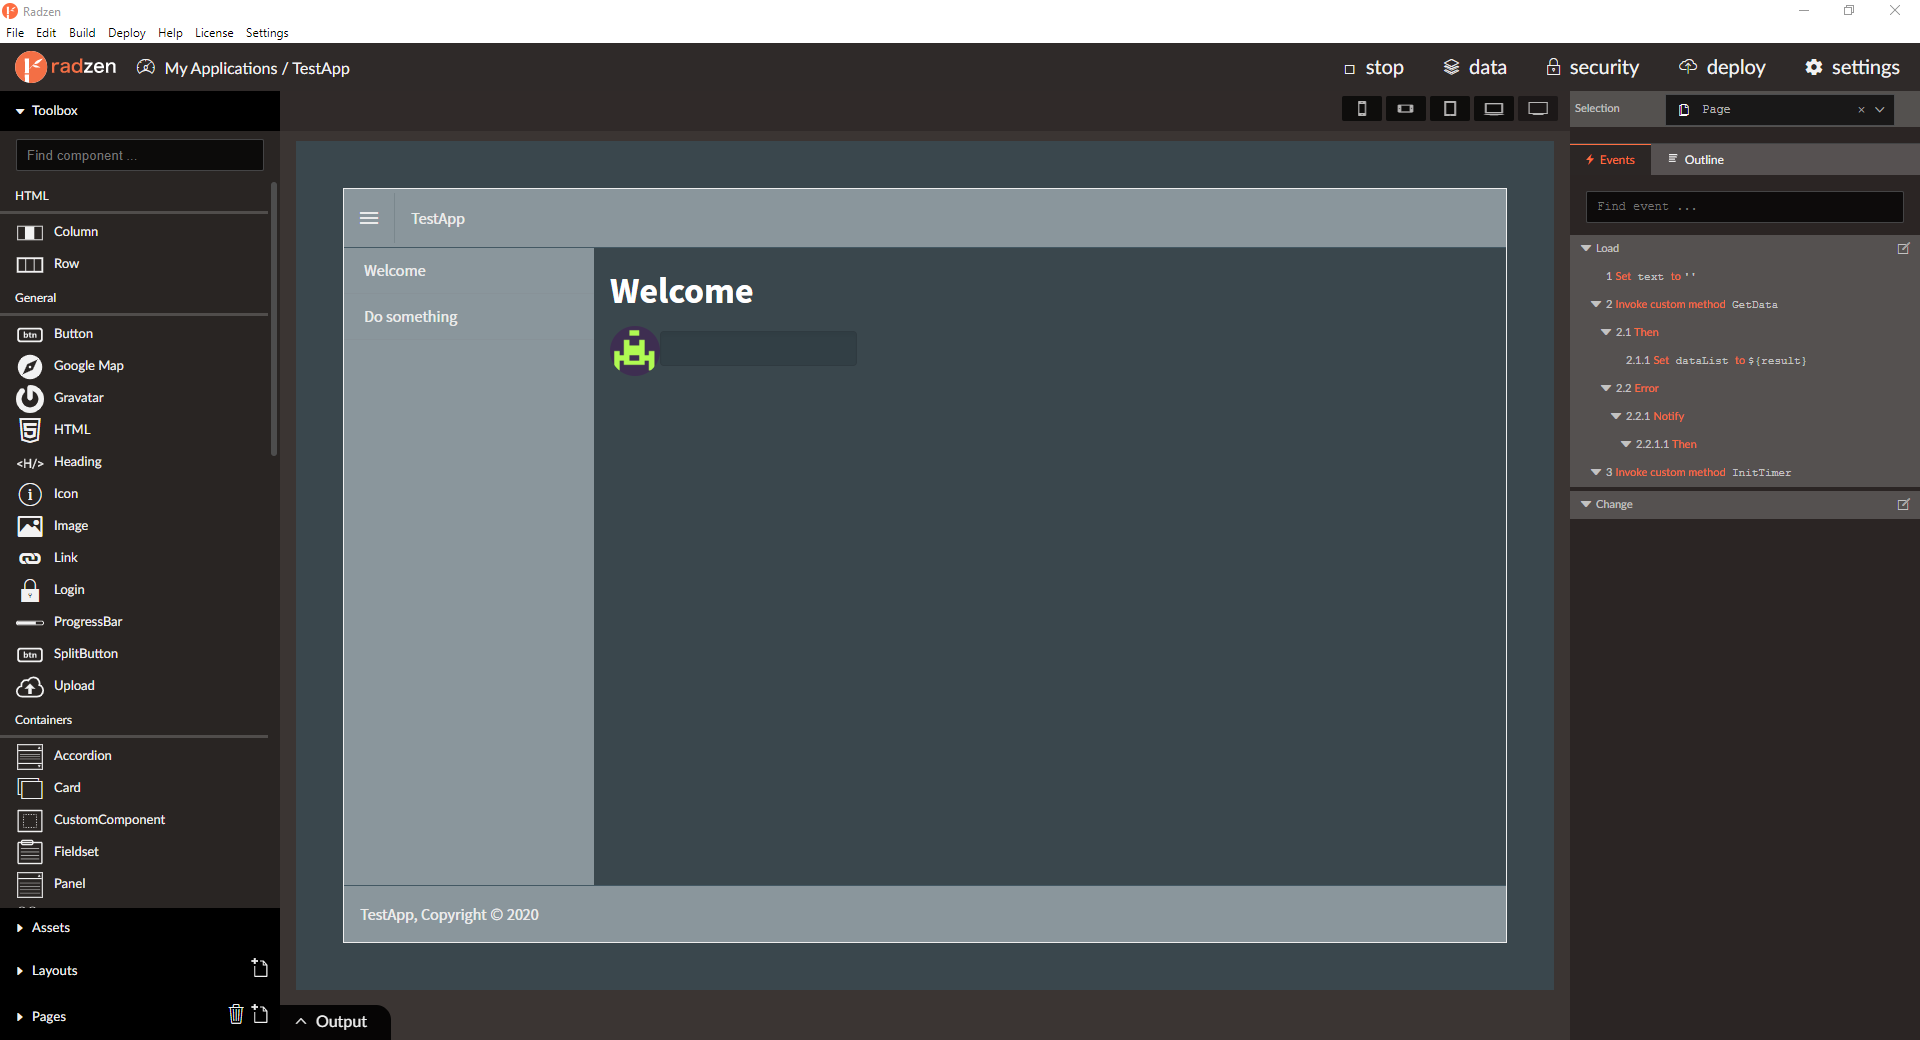
\includegraphics[width=\textwidth]{img/radzen_overview}
  \caption{\label{fig-radzen_overview}Radzen - \gls{UI}-Designer}
\end{figure}

\noindent Das in \Cref{fig-radzen_overview} abgebildete Beispielprojekt kann durch einen Klick auf den \enquote{run}-Knopf ausgeführt werden. Dadurch wird der Code generiert und die Seite angezeigt (\Cref{fig-radzen_example}). Der \enquote{Gravatar} kann dynamisch durch Ändern der E-Mail-Adresse des Textfeldes geändert werden.

\begin{figure}[htbp]
  \centering
  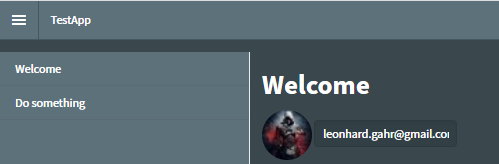
\includegraphics[width=0.65\textwidth]{img/radzen_example}
  \caption{\label{fig-radzen_example}Radzen - Gravatar Beispiel}
\end{figure}

\noindent Das von Radzen erstellte Projekt lässt sich mit \gls{visual-studio} öffnen. In \gls{visual-studio} lassen sich eigene Klassen oder \enquote{Custom Components} erstellen. Ein \enquote{Custom Component} kann innerhalb von Radzen wiederum eingebunden und auf der Seite angezeigt werden. Die Komponente selbst wird von Radzen nicht automatisch generiert, sodass sie auch nicht überschrieben wird. Alle Seiten jedoch, die mit Radzen angelegt werden, werden beim Start des Projekts wieder neu generiert.\\
\enquote{Custom Components} dienen der Implementierung von Dingen, die Radzen selbst nicht unterstützt.

\newpage
\subsection{Workorder Planner}
Nach der Einarbeitung in ein Radzen Beispielprojekt kann der Workorder Planner selbst umgesetzt werden. Der erste Schritt hierbei ist die Auswahl der richtigen Darstellungsweise und Bibliothek. Dabei stehen die Darstellungsarten Gantt und Scheduler zur Auswahl, die beide von der \enquote{Syncfusion Blazor
component library}\citetitlerefFootnote{syncfusion.2020a} bereitgestellt werden. Da Syncfusion eine Bibliothek für Blazor ist, ist die Anbindung kein Problem, da Syncfusion lediglich in \gls{visual-studio} als Bibliothek hinzugefügt werden muss. Der Syncfusion Beispielcode ist ausreichend, um erste Informationen zu erhalten.

\subsubsection{Gantt-Chart}
Ein Gantt Chart erfüllt visuell die Anforderungen an die Anzeige. Als Task werden die Arbeitsaufträge aus der Datenbank angezeigt. Da die Datenbankverbindung extern geschehen soll, wird als Datenquelle vorübergehend eine JSON-Datei verwendet, dessen Struktur im Code Auszug \ref{listing_json-source-file} dargestellt ist.

\begin{lstlisting}[language={JavaScript},
frame=single,
framexleftmargin=15pt,
style=algoBericht,
label={listing_json-source-file},
captionpos=b,
caption={Struktur der Quell-JSON-Datei}]
[
  {
    "Id": 1,
    "Name": "SomeName",
    "StartDate": "2019-04-23",
    "Duration": "5",
    "Status": "c"
  },
  {
    "Id": 2,
    "Name": "Create Something",
    "StartDate": "2019-04-07",
    "Duration": "2",
    "Status": "r"
  },
  ...
]
\end{lstlisting}

\newpage\noindent Diese Daten werden geladen und der Blazor Komponente bereitgestellt, die bei jedem Laden der Seite diese Daten neu anfordert. Der Code Auszug \ref{listing_gantt-component} zeigt die Definition der Blazor Komponente für ein Gantt-Diagramm. Diese Komponente wird als \enquote{Custom Component} bei Radzen hinzugefügt.

\begin{lstlisting}[language={XML},
frame=single,
framexleftmargin=15pt,
style=algoBericht,
label={listing_gantt-component},
captionpos=b,
caption={Custom Gantt Component}]
@using Syncfusion.Blazor.Gantt
@using MesPortal.Services

<SfGantt DataSource="@TaskCollection" Height="100%" Width="100%"
    Toolbar="@(new List<string> {"ZoomIn", "ZoomOut", "ZoomToFit"})"
    TreeColumnIndex="1" AllowFiltering="true"
    ProjectStartDate="@ProjectStart" ProjectEndDate="@ProjectEnd">

    <GanttTaskFields Id="Id" Name="Name" StartDate="StartDate"
        EndDate="EndDate" Duration="Duration" Progress="Progress"
        Notes="Status">
    </GanttTaskFields>
</SfGantt>

@code{
    public DateTime ProjectStart = new DateTime(2019, 3, 24);
    public DateTime ProjectEnd = new DateTime(2020, 12, 28);
    public List<GanttData.WorkOrder> TaskCollection { get; set; }

    protected override void OnInitialized()
    {
        TaskCollection = GanttData.LoadJson();
    }
}
\end{lstlisting}

\noindent Wenn die Syncfusion-Abhängigkeiten eingebunden sind, wird das Radzen Projekt gestartet. \Cref{fig-wo_planner_gantt} zeigt die Komponente, nachdem sie geladen ist. Jeder Task stellt hier einen Arbeitsauftrag dar. Es ist zu erkennen, dass bei wenigen Arbeitsaufträgen eine übersichtliche Anzeige gewährleistet ist. Betrachtet man nun jedoch, dass in einer Anlage mehrere Hundert Arbeitsaufträge geplant sein können, stellt sich heraus, dass ein Gantt-Diagramm nicht die richtige Darstellungsweise ist, da für jeden Arbeitsauftrag eine neue Zeile im Diagramm angelegt wird. Dies entspricht auch nicht der eigentlichen Anforderung (siehe \Cref{fig-mes_portal_workorder-planner}). Diese Tatsache ist leider erst spät aufgefallen, da nach ersten Eindrücken das Gantt-Diagramm nach der passenden Lösung ausgesehen hat. Die alternative Darstellungsweise ist der von Syncfusion bereitgestellte Scheduler.

\begin{figure}[htbp]
  \centering
  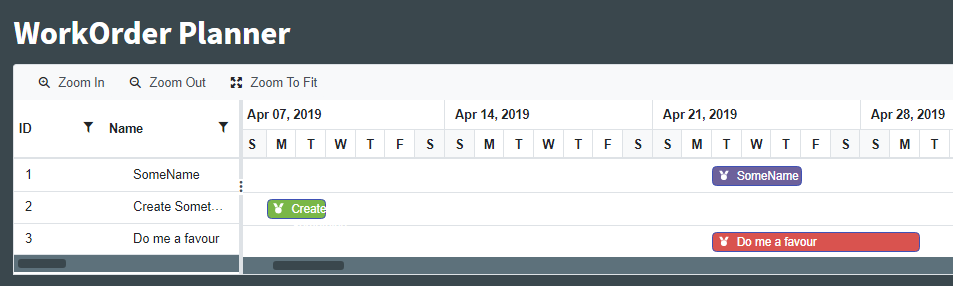
\includegraphics[width=0.9\textwidth]{img/wo_planner-gantt}
  \caption{\label{fig-wo_planner_gantt}MES-Portal Workorder Planner (Gantt)}
\end{figure}

\subsubsection{Scheduler}
Der zweite Ansatz der Umsetzung des Workorder Planners mit einem Scheduler kann aus zeitlichen Gründen nicht im Radzen Projekt übernommen werden. \Cref{fig-wo_planner_timeline} zeigt ein Beispiel von Syncfusion\citetitlerefFootnote{syncfusion.2020b} zu einem Scheduler Timeline Diagramm mit Gruppierung. Diese Ansicht passt genau auf die Anforderungen, unter Berücksichtigung, dass die Höhe der einzelnen Gruppen angepasst werden kann, damit mehrere Arbeitsaufträge gleichzeitig in einer Gruppe angezeigt werden. Der Dokumentation zufolge ist dies möglich, es kann aber nicht im Rahmen dieser Arbeit umgesetzt werden.

\begin{figure}[htbp]
  \centering
  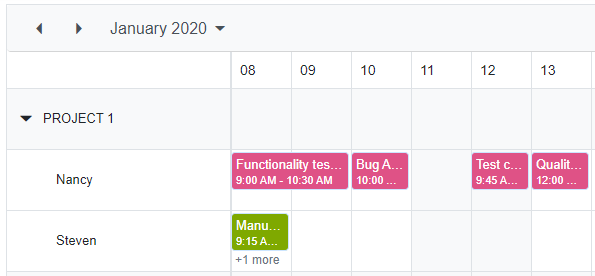
\includegraphics[width=0.8\textwidth]{img/wo_planner-timeline}
  \caption{\label{fig-wo_planner_timeline}Syncfusion Scheduler Timeline Gruppierung Beispiel}
\end{figure}

\section{Schwierigkeiten mit Radzen}
Der Funktionsumfang von Radzen ist sehr groß, weshalb Radzen mehr als nur ein Framework ist. In diesem Fall zieht Radzen den Nachteil mit sich, dass während der Entwicklung eine Internetverbindung benötigt wird.\\
Bei Siemens findet die Entwicklung von Produkten zu \gls{OP EX PH} normalerweise auf \glspl{vm} auf einem \gls{ESXi} Server statt. Sicherheitshalber hat dieser \gls{ESXi} Server keine Anbindung an das Internet und ist nur aus dem internen Siemens-Netzwerk erreichbar. Daher kann Radzen nicht auf diesen \glspl{vm} laufen und muss lokal verwendet werden. Dafür muss eine lokale \gls{vm} installiert werden, auf der \gls{OP EX PH} läuft. Außerdem muss der PC leistungsstark genug sein, um ein solches System einwandfrei am Laufen zu halten. Dies ist durch die Ausbildungslaptops der Siemens AG Karlsruhe nicht standardmäßig gegeben. Dadurch, dass ein Ersatzgerät organisiert werden muss, tritt zusätzlich eine Verzögerung bei der Entwicklung auf.

\section{Zukünftige Entwicklungen}
Im Rahmen der Arbeit kann nur der Workorder Planner teilweise entwickelt werden. Die zukünftige Entwicklung zu diesem Projekt schließt den Workorder Planner mit der Scheduler Timeline Komponente von Syncfusion ab.\\
Die Einarbeitung in den Test Manager ist abgeschlossen und die Entwicklung kann nach Abschluss des Workorder Planners beginnen.

\chapter{Reflexion}
Trotz der nicht vollständig abgeschlossenen Projekte wurde die vierte Praxisphase bei der Siemens AG erfolgreich abgeschlossen. Das erworbene Wissen und die angefangenen Arbeiten dienen als Grundlage für weitere Entwicklungen im Bereich des MES Portals und weiteren Produkten bezüglich \gls{OP EX PH}. Eine Portierung weiterer Produkte von \gls{VB}6 in webbasierte Technologien ist absehbar. In diesem Bereich dienen Erfahrungen mit neuen Frameworks als Grundlage für den schnelleren Erfolg weiterer Entwicklungen.

\section{Informationsgewinn \& Lernerfolge}
Die Analyse des \gls{VB}6 Codes (siehe \Cref{subsec_backend}) ermöglichte Einblicke in das Verstehen von fremden Code in einer fremden Programmiersprache, ohne mit dieser Sprache selbst programmieren zu müssen. Aufgrund des konstanten Wandels und der stetigen Weiterentwicklung von Technologien, wird diese Fähigkeit auch in Zukunft Anwendung finden.\\
Aus programmiertechnischer Sicht konnte die neue Web Framework Blazor kennengelernt werden, das im Jahr 2020 sehr großen Anklang gefunden hat und eine neue alternative zu JavaScript basierten Frameworks wie Angular oder React ist. Des Weiteren wurde mit C\myHashtag\ \gls{full-stack} entwickelt und der Umgang mit OracleSQL wurde vertieft.\\
Für das kollaborative Arbeiten wurde das Versionskontrollsystem GIT verwendet, was das am weitesten verbreitete Versionskontrollsystem ist (vgl. \cite{datanyze.2020a}, unter der Beachtung, dass z. B. Github auf GIT basiert).

\section{Überschneidung mit Vorlesungsinhalten}
Durch die detaillierten Einblicke in Datenbanksysteme und in die \gls{SQL} durch die Vorlesung \enquote{Datenbanken} des dritten und vierten Semesters, konnte die Arbeit mit OracleSQL stark erleichtert werden.\\
Das Arbeiten mit neuen Technologien und generelle Arbeit in der Softwareentwicklung wurde in der Vorlesung \enquote{Software Engineering I} behandelt. Für die Vorlesung \enquote{Software Engineering II} konnten hier sinnvolle Kenntnisse angeeignet werden.\\
Obwohl es sich um ein Webentwicklungsprojekt handelt, konnte das Wissen aus den Vorlesungen \enquote{Webengineering I + II} hier nicht angewandt werden. Der Grund dafür ist, dass Blazor nicht wie andere Web Technologien funktioniert und in diesem Sinn nicht in den Vorlesungen behandelt wurde. Durch Radzen wurde die Arbeit mit HTML, CSS und JavaScript abgenommen.

% begin of appendix
\clearpage
\appendix
\chapter{Praxisbericht T3\textunderscore 2000A (Kapitel 2) - Leonhard Gahr}\label{appendix_T2000_gahr}
%\includepdf[pages={12-12},pagecommand={}]{appendix/T2000A_Gahr.pdf}
\clearpage

\cleardoublepage\phantomsection\addcontentsline{toc}{chapter}{Literaturverzeichnis}
\def\refname{Literaturverzeichnis}
\printbibliography

\newpage
\listoftodos
\end{document}